% Paper template for TAR 2016
% (C) 2014 Jan Šnajder, Goran Glavaš, Domagoj Alagić, Mladen Karan
% TakeLab, FER

\documentclass[10pt, a4paper]{article}

\usepackage{tar2016}

\usepackage[utf8]{inputenc}
\usepackage[pdftex]{graphicx}
\usepackage{booktabs}
\usepackage{amsmath}
\usepackage{amssymb}

\graphicspath{{img/}}

\title{Semantic Textual Similarity using deep learning}

\name{Bruno Gavranovic, Neven Miculinic, Stipan Mikulic}

\address{
University of Zagreb, Faculty of Electrical Engineering and Computing\\
Unska 3, 10000 Zagreb, Croatia\\
\texttt{\{bruno.gavranovic,neven.miculinic,stipan.mikulic\}@fer.hr}\\
}


\abstract{
In this paper we present our work on Semantic Textual Similarity (STS) problem during Text analysis and retrival (TAR) class at FER.
STS measures semantic similarity between two sentences.
We use two approaches: an SVM model with feature preprocessing and a deep learning model trained on a language modelling task.
Datasets were obtained using human annotators and their average semantic similarity score is given.
We use both Pearson and Spearman correlation coefficient in our analysis and achieve 1.000, and 1.000 on our test set respectively.
}

\begin{document}

\maketitleabstract

\section{Introduction}

\begin{verbatim}
Two dogs play in the grass.
Two dogs playing in the snow.
\end{verbatim}

At the heart of STS, semantic textual similarity, is assigning numerical score on two text similarity. By text, it could mean full document, paragraph, or in this paper's case only one sentence. Beginning quote showcases one such sentance pairs, where human annotators rated 2.8 semantically similar on 0-5 scale, where 0 mean full semantic dissimilarity, and 5 full equivalence with various shades in between. Full score semantics you can read in table~\ref{tab:sts-score}


STS developed system and techniqus have many further applications, transfer learning of sorts. Machine translation(MT), Summarization, Generation and Question Answering(QA) are some of them. Often new techniques invented in STS context generlize to earlier mentioned domains, as well as NLP fiels as a whole.


\begin{table*}
\caption{STS score description, adapted from~\citep{agirre2016semeval}}
\label{tab:sts-score}
\begin{center}
\begin{tabular}{llr}
\toprule
Score & Explanation\\
\midrule
5 & \textit{Two sentences are completely equivalent}\\
& The bird is bathing in the sink\\
& Birdie is washing itself in the water basin.\\
\midrule
4 & \textit{The two sentences are mostly equivalent, but some unimportant details differ}\\
& In May 2010, the troops attempted to invade
Kabul. \\
& The US army invaded Kabul on May 7th last
year, 2010.\\
\midrule
3 & \textit{The two sentences are roughly equivalent, but some important information differs/missing.}\\
& John said he is considered a witness but not a
suspect.\\
& ``He is not a suspect anymore.'' John said.\\
\midrule
2 & \textit{The two sentences are not equivalent, but share some details.} \\
&They flew out of the nest in groups. \\
&They flew into the nest together. \\
\midrule
1 & \textit{The two sentences are not equivalent, but are on the same topic.}\\
& The woman is playing the violin.\\
& The young lady enjoys listening to the guitar.\\
\midrule
0 & \textit{The two sentences are completely dissimilar.}\\
& John went horse back riding at dawn with a whole group of friends.\\
& Sunrise at dawn is a magnificent view to take in if you wake up early enough for it.\\
\bottomrule
\end{tabular}
\end{center}
\end{table*}

\section{Related work}

STS has short and fruitful history, one with many ideas flying around. In its current form it appeared in 2012, on SemVal~\citep{agirre2012semeval} as task 6.  In 2012, the best system~\citep{bar2012ukp} used lexical similarity and Explicit Semantic Analysis(ESA)~\citep{gabrilovich2007computing}. Following year Latent Semantic Analysis(LSA)~\citep{deerwester1990indexing} model~\citep{han2013umbc} with additional external information sources, WordNet and n-gram matching technique.

Following two years~\citep{sultan2014dls} and~\citep{sultan2015dls} dominate the competition with new algorithm -- they align the words between new sentences. Other notable approaches come from logic side, its representative paper being~\citep{beltagy2014probabilistic}.

\section{Extent of the paper}

Our contribution consists of implementation of two machine learning models: SVM model and a deep learning model.

\subsection{SVM}

\subsection{Deep learning}

\begin{figure}
\begin{center}
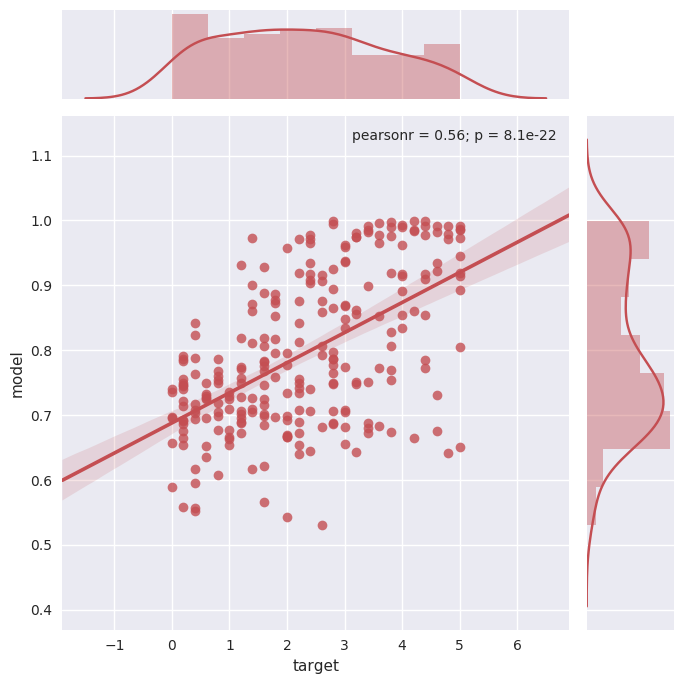
\includegraphics[width=\columnwidth]{only_2nd_layer.png}
\caption{Depiction of blabla}
\label{fig:lstm_2nd_layer}
\end{center}
\end{figure}

\subsection{Tables}

There are two types of tables: narrow tables that fit into one column and a wide table that spreads over both columns.

\subsubsection{Narrow tables}

Table~\ref{tab:narrow-table} is an example of a narrow table. Do not use vertical lines in tables -- vertical tables have no effect and they make tables visually less attractive. We recommend using \textit{booktabs} package for nicer tables.

\begin{table}
\caption{This is the caption of the table. Table captions should be placed \textit{above} the table.}
\label{tab:narrow-table}
\begin{center}
\begin{tabular}{ll}
\toprule
Heading1 & Heading2 \\
\midrule
One & First row text \\
Two   & Second row text \\
Three   & Third row text \\
      & Fourth row text \\
\bottomrule
\end{tabular}
\end{center}
\end{table}

\subsection{Wide tables}

Table~\ref{tab:wide-table} is an example of a wide table that spreads across both columns. The same can be done for wide figures that should spread across the whole width of the page.

\begin{table*}
\caption{Wide-table caption}
\label{tab:wide-table}
\begin{center}
\begin{tabular}{llr}
\toprule
Heading1 & Heading2 & Heading3\\
\midrule
A & A very long text, longer that the width of a single column & $128$\\
B & A very long text, longer that the width of a single column & $3123$\\
C & A very long text, longer that the width of a single column & $-32$\\
\bottomrule
\end{tabular}
\end{center}
\end{table*}

\section{Math expressions and formulas}

Math expressions and formulas that appear within the sentence should be written inside the so-called \emph{inline} math environment: $2+3$, $\sqrt{16}$, $h(x)=\mathbf{1}(\theta_1 x_1 + \theta_0>0)$. Larger expressions and formulas (e.g., equations) should be written in the so-called \emph{displayed} math environment:

\[
b^{(i)}_k = \begin{cases}
1 & \text{if
    $k = \text{argmin}_j \| \mathbf{x}^{(i)} - \mathbf{\mu}_j \|,$}\\
0 & \text{otherwise}
\end{cases}
\]

Math expressions which you reference in the text should be written inside the \textit{equation} environment:

\begin{equation}\label{eq:kmeans-error}
J = \sum_{i=1}^N \sum_{k=1}^K
b^{(i)}_k \| \mathbf{x}^{(i)} - \mathbf{\mu}_k \|^2
\end{equation}

Now you can reference equation \eqref{eq:kmeans-error}. If the paragraph continues right after the formula

\begin{equation}
f(x) = x^2 + \varepsilon
\end{equation}

\noindent like this one does, use the command \emph{noindent} after the equation to remove the indentation of the row.

Multi-letter words in the math environment should be written inside the command \emph{mathit}, otherwise \LaTeX{} will insert spacing between the letters to denote the multiplication of values denoted by symbols. For example, compare
$\mathit{Consistent}(h,\mathcal{D})$ and\\
$Consistent(h,\mathcal{D})$.

If you need a math symbol, but you don't know the corresponding \LaTeX{} command that generates it, try
\emph{Detexify}.\footnote{\texttt{http://detexify.kirelabs.org/}}

\section{Referencing literature}

References to other publications should be written in brackets with the last name of the first author and the year of publication, e.g., \citep{chomsky-73}.  Multiple references are written in sequence, one after another, separated by semicolon and without whitespaces in between, e.g., \citep{chomsky-73,chave-64,feigl-58}. References are typically written at the end of the sentence and necessarily before the sentence punctuation.

If the publication is authored by more than one author, only the name of the first author is written, after which abbreviation \emph{et al.}, meaning \emph{et alia}, i.e.,~and others is written as in \citep{johnson-etc}. If the publication is authored by only two authors, then the last names of both authors are written \citep{johnson-howells}.

If the name of the author is incorporated into the text of the sentence, it should not be in the brackets (only the year should be there). E.g.,~``\citet{chomsky-73}
suggested that \dots''. The difference is whether you reference the publication or the author who wrote it.

The list of all literature references is given alphabetically at the end of the paper. The form of the reference depends on the type of the bibliographic unit: conference papers,
\citep{chave-64}, books \citep{butcher-81}, journal articles
\citep{howells-51}, doctoral dissertations \citep{croft-78}, and book chapters \citep{feigl-58}.

All of this is automatically produced when using BibTeX. Insert all the BibTeX entries into the file \texttt{tar2016.bib}, and then reference them via their symbolic names.

\section{Conclusion}

Conclusion is the last enumerated section of the paper. It should not exceed half of a column and is typically split into 2--3 paragraphs. No new information should be presented in the conclusion; this section only summarizes and concludes the paper.

\section*{Acknowledgements}

If suitable, you can include the \textit{Acknowledgements} section before inserting the literature references  in order to thank those who helped you in any way to deliver the paper, but are not co-authors of the paper.

\bibliographystyle{tar2016}
\bibliography{tar2016}

\end{document}
